\chapter{Problem Statement}
\label{Problem_Statement}
\thispagestyle{empty}

In this chapter we provide a mathematical formulation of the problem we tackle in this thesis.
In the first part of this chapter, we define the environment as a Markov Decision Process (MDP).
As said before, the problem of designing an agent able to perform a race on track with human-like skills can be divided into two sub goals. The first is purely based on imitation learning, where the agent learns to follow the reference trajectory, whilst in the second goal a new agent is built upon the previous one and learns to improve the imitating policy.


\section{Environment Formulation}

The racing of a car on the track can be represented as an MDP, where the state corresponds to the situation of the car on the track, $\boldsymbol s \in \mathbb{R}^n,$ where $n$ is the number of features that we will define in chapter \ref{Methods}; the action $\boldsymbol a \in \mathbb{R}^3$ is a vector of three continuous variables, defined as: steering with $ a_s \in [-1,1] $, where positive values mean steer left while negative ones mean steer right, throttle with $ a_t \in [0,1] $ and brake with $ a_b \in [0,1] $. These ranges of values are given by the environment. We assume the MDP to be deterministic such that the transition probability distribution is  $p(\boldsymbol s_{t+1}=\boldsymbol s|\boldsymbol a_t, \boldsymbol s_t) = \delta(\boldsymbol s - f(\boldsymbol a_t,\boldsymbol s_t)),$ where $\delta(\boldsymbol s)$ is the Dirac Delta function and $f(\cdot)$ is a function implemented by the simulator. Thus, the transition function is embedded in the simulator.
The MDP has one starting start $S_0$ but has many terminal states. The terminal state is the final state of the episode. In our case, two situations can occur: the car reaches the endline of the track, which is considered as a success, receiving a reward of $0$ or the car goes out of track, which is considered as failure and the agent receives a negative reward signal. For intermediate steps the reward is given by a \textit{reward function} $r(\cdot),$ which will be defined in Section \ref{sec:reward_function}.
We represent the expert demonstrations as a set $\mathcal{D}=\{\boldsymbol l_i|i= 0,..,m\}$ where $m$ is the number of sampled trajectories from this MDP and $\boldsymbol l_i$ is a sequence of states and actions $\boldsymbol s_0^i,\boldsymbol a_0^i,\boldsymbol s_1^i,\boldsymbol a_1^i,...,\boldsymbol s^i_{n_i}$, where $\boldsymbol s^i_{n_i}$. It is important to note that the time-lengths of these trajectories are known.
We have access to the environment through observations $\boldsymbol x \in X$, where $\boldsymbol x$ is a vector of features that we will define in \ref{sec:obs}.

Then, we define a \textit{reference trajectory} $\boldsymbol l_{ref}$ as the shortest sequence of state-action belonging to $\mathcal{D}$, i.e. the one with the shortest time.
The reward function $r(\cdot)$ is expressed in terms of the reference trajectory. When the agent performs worse than the expert it receives a negative reward signal, whereas when it does better it receives a positive one.

\section{Reference Trajectory Following}
\label{ref_follow}

In the imitation learning problem, the parametric policy $\psi_{\boldsymbol \omega}$, with parameter vector $\boldsymbol \omega$, seeks to minimize the difference between the agent trajectory and the human demonstration. The trajectory divergence is defined as:

\begin{equation}\mathcal{L}_\tau = \frac{1}{|\tau|} \sum_{s \in \tau} {\lVert}{s - l_\perp}{\rVert}^2, \end{equation} where $\tau$ is the trajectory, $|\tau| = n$ is the trajectory length and $l_\perp$ is the projection of the state on the reference trajectory.

However, this loss is not used directly for the optimization of the policy (indeed, it does not depend on $\boldsymbol \omega$) but it is implicit in the policy $\psi_{\boldsymbol \omega}$, with parameters vector $\theta$. Therefore, the rules of the policy are parametrized by $\boldsymbol \omega$ and are expressed so as to minimize $\mathcal{L}_\tau.$ The goal of the problem, thus, is to find the parameter vector $\boldsymbol \omega$ that allows the agent to perform a lap on the track that minimizes $\mathcal{L}_\tau$. Finding the optimal $\boldsymbol \omega^*$ can be cast to an RL policy optimization problem in which the objective function to maximize is the expected return obtained by following 
\begin{equation}J(\boldsymbol \omega)=\int_{\mathcal{T}} p(\tau|\boldsymbol \omega)R(\tau)d \tau,\end{equation}
where $p(\tau|\boldsymbol \omega)$ is the trajectory density function and $R(\tau)$ is the reward of the trajectory $\tau$.

Note that by using a reward function consistent with the reference trajectory, the maximization of $J(\boldsymbol \omega)$ implicitly leads to the minimization of $\mathcal{L}_\tau.$
However, the policy $\psi_{\boldsymbol \omega}$, by design cannot perform better than the expert demonstration. For this reason, the policy $\psi_{\boldsymbol \omega}$ will be used as a base for the next step.







\section{Reference Trajectory Improvement}
\label{ref_improve}

Once the first goal is achieved, the imitating policy $\psi_{\boldsymbol \omega^*}$ is kept fixed. Upon this, a new agent is built. The goal of this second policy $\pi_{\boldsymbol{\theta}}$ is to improve the performance, i.e., the lap-time, by correcting the behaviours of the former policy. The objective function

\begin{equation}J(\boldsymbol \theta)=\int_{\mathcal{T}} p(\tau|\boldsymbol \theta)R(\tau)d \tau\end{equation}

corresponds to the expected return obtained by following the policy $\pi_{\boldsymbol{\theta}}$. The maximization of $J(\boldsymbol \theta)$, through RL policy optimization, results in finding the optimal policy parameter $\boldsymbol \theta^*$. 


Fig.\ref{fig:diagram3} is a schematic representation of the interactions between the policy $\pi_{\boldsymbol{\theta}}$, the environment and the optimized imitating policy $\psi_{\boldsymbol \omega^*}$.

The environment, after receiving an action $A_{t-1}$, gives back the observation $X_t$. Some of the features which compose $X_t$ will be useful to the imitating policy, whilst others to the improving policy. For this reason, $X_t$ is split into two vectors $X_t^{\psi}$ and $X_t^{\pi}$: the former is given as input to the imitating policy, while the latter is processed from a feature extractor $f_e$ which receives the observation and produces a vector of features $\Phi_t$, i.e., $f_e(X_t^{\pi})= \Phi_t.$
The imitating policy computes an action $A_t^{\psi_{\boldsymbol \omega^*}}$ aimed at following the reference trajectory.
Then, by combining the features $\Phi_t$ with the action $A_t^{\psi_{\boldsymbol \omega^*}}$, a new state $S_t$ is produced.
The improving policy $\pi_{\boldsymbol{\theta}}$ receives the state $S_{t+1}$ and computes a correction, or delta action $A_{t+1}^{\pi_{\boldsymbol{\theta}}}$ that, combined with $A_{t+1}^{\psi_{\boldsymbol \omega^*}}$, produces the final action $A_{t+1}$.


\begin{figure}
    \centering
 	  \captionsetup{width=10cm}
      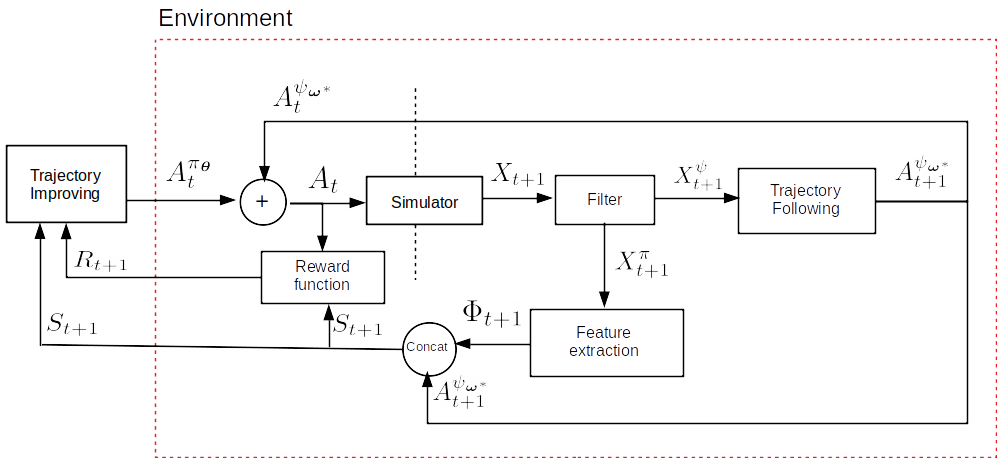
\includegraphics[width=14cm]{./img/diagram_new}
     \caption{Improving Policy, imitating Policy and Environment interface. The dashed line stands for a time step advance}
   \label{fig:diagram3}
  \end{figure}